%
% avaliacao.tex
% Capítulo 5 — Avaliação e Resultados
%
% DADOS REAIS: extraídos da BD PostgreSQL em produção (2026-06-14) e do CSV do questionário (n=12).
% SUS calculado pelo método Brooke (1996).
%
\chapter{Avaliação e Resultados}
\label{cha:avaliacao}

Este capítulo reporta a avaliação preliminar do \emph{Play4Change} sob dois ângulos: a integridade do sistema de geração de conteúdo (§\ref{sec:integridade-geracao}), com base nos registos da base de dados em produção e do Prometheus; e o comportamento dos utilizadores (§\ref{sec:comportamento-utilizadores}), triangulando os dados comportamentais da BD com um questionário pós-utilização.

% ─────────────────────────────────────────────────────────────────────────────
\section{Metodologia de avaliação}
\label{sec:metodologia-avaliacao}
% ─────────────────────────────────────────────────────────────────────────────

O questionário ($n=12$) foi administrado remotamente após exploração livre do protótipo. Organizava-se em quatro secções: perfil do respondente; usabilidade e envolvimento em escala de Likert; os dez itens da \emph{System Usability Scale} (SUS)~\cite{brooke1996sus}; e questões abertas. Os itens foram cotados pelo método de Brooke~\cite{brooke1996sus}, dando uma escala de 0 a 100; pontuações acima de 68 estão acima da média histórica e, segundo a escala de adjetivos de Bangor et al.~\cite{bangor2008empirical}, pontuações acima de aproximadamente 71 são qualificadas como ``boas'' (\emph{good}) e acima de 85 como ``excelentes'' (\emph{excellent}).

Os dados comportamentais cobrem o último ciclo de testes contínuo após o derradeiro \emph{reset} de desenvolvimento.\footnote{A BD sofreu limpezas de estado intencionais durante o desenvolvimento (migrações Flyway V1--V28+). Os valores da Tabela~\ref{tab:stats-gerais} representam o \emph{snapshot} do último ciclo, não o total histórico acumulado desde o início do projecto.} O rácio entre os 15 utilizadores registados na BD e os 12 questionários preenchidos explica-se por utilizadores do ciclo anterior que responderam ao formulário mas não voltaram a interagir com o protótipo após a reinicialização. Os doze respondentes (P01--P12) foram identificados no momento de resposta ao questionário, o que permitiu associar cada resposta ao respectivo utilizador na BD; é esta associação que sustenta o cruzamento entre pontuação SUS e dados comportamentais na Secção~\ref{ssec:sus}. Os três utilizadores registados na BD sem questionário associado não são incluídos nessa análise cruzada.

% ═════════════════════════════════════════════════════════════════════════════
\section{Integridade do sistema de geração}
\label{sec:integridade-geracao}
% ═════════════════════════════════════════════════════════════════════════════

Os seis tópicos criados durante o período de avaliação transitaram todos para o estado \texttt{ACTIVE}, sem nenhum em \texttt{FAILED} --- o que é consistente com o pipeline de quatro fases (INGESTION, ANALYSIS, GENERATION, INDEXING) ter operado dentro dos parâmetros de fiabilidade definidos, ainda que uma amostra de seis tópicos seja demasiado pequena para uma conclusão estatisticamente robusta sobre a taxa de falhas do pipeline. A Tabela~\ref{tab:timing-geracao} reporta os tempos de transição reais registados na tabela \texttt{topic\_phase\_log}.

\begin{table}[htbp]
	\centering
	\small
	\begin{tabular}{l r r p{5cm}}
		\toprule
		\textbf{Fase} & \textbf{Mín.} & \textbf{Máx.} & \textbf{Nota} \\
		\midrule
		INGESTION $\to$ ANALYSIS   & 13\,ms           & 95\,s    & URL (instantâneo) vs PDF (extracção) \\
		ANALYSIS $\to$ GENERATION  & 10\,ms           & 65\,ms   & \\
		GENERATION $\to$ INDEXING  & 6,3\,s           & 11,3\,s  & Chamada LLM (\texttt{mistral-small-latest}) \\
		INDEXING $\to$ ACTIVE      & 54\,s            & 121\,s   & \emph{Embeddings} batch (58 templates) \\
		\midrule
		\textbf{Pipeline completo} & \textbf{$\approx$1\,min} & \textbf{$\approx$4\,min} & 6/6 tópicos ACTIVE; 0 FAILED \\
		\bottomrule
	\end{tabular}
	\caption[Tempos reais de transição do pipeline de geração (fonte: \texttt{topic\_phase\_log})]{Tempos de transição entre fases para os seis tópicos criados durante o período de avaliação, extraídos diretamente da tabela \texttt{topic\_phase\_log}. A variação na fase INGESTION reflete a diferença entre fontes URL e PDF.}
	\label{tab:timing-geracao}
\end{table}

A integridade das 58 \emph{task templates} validadas é garantida por dois mecanismos: validação campo a campo do JSON produzido pelo LLM (com retentação automática via \emph{schema reminder} em caso de falha) e um \emph{circuit breaker} Resilience4j que interrompe o pipeline se a taxa de falhas ultrapassar 50\% numa janela de 10 chamadas. Nenhum alerta Prometheus foi ativado durante o período de avaliação, o que é coerente com a ausência de relatos de erros de geração.

A latência de inferência medida pelo Prometheus manteve-se dentro do \emph{timeout} de 60\,s por chamada (P95\,=\,14,26\,s para GENERATION; P95\,=\,4,04\,s para ANALYSIS).

Os 33 ramos distintos servidos a 55 sessões mostram uma distribuição desigual: o ramo mais reutilizado serviu 22 das 55 sessões (40\%), uma concentração que indica que a deduplicação vectorial (Secção~\ref{cha:desenvolvimento}) está a agrupar correctamente um padrão de erro particularmente comum num único ramo partilhado, em vez de gerar conteúdo redundante para cada ocorrência. Os restantes 32 ramos, cada um servindo entre 1 e poucas sessões, preservam diversidade para os padrões de erro menos frequentes.

% ═════════════════════════════════════════════════════════════════════════════
\section{Comportamento dos utilizadores}
\label{sec:comportamento-utilizadores}
% ═════════════════════════════════════════════════════════════════════════════

% ─────────────────────────────────────────────────────────────────────────────
\subsection{Visão geral}
\label{ssec:dados-comportamentais}
% ─────────────────────────────────────────────────────────────────────────────

A Tabela~\ref{tab:stats-gerais} reporta os indicadores globais extraídos da BD. Os 104/105 acertos finais (99\%) não indicam facilidade excessiva --- indicam a eficácia do ciclo adaptativo: as 55 sessões geradas confirmam que uma parcela significativa de tarefas envolveu pelo menos uma resposta errada seguida de reforço. O número de sessões (55) excede o número de tarefas com pelo menos um erro inicial (25) porque uma única tarefa falhada pode originar mais do que uma sessão: se o utilizador falhar também as subtarefas de reforço, o sistema encadeia uma segunda sessão de \emph{struggle} a partir da mesma tarefa original antes de, no limite de profundidade, escalar para uma sessão de explicação por IA --- pelo que a contagem de sessões reflecte eventos de falha (incluindo reincidências), não tarefas distintas.

Quanto aos distintivos: a taxa de aprovação de 100\% não constitui evidência independente da eficácia do limiar $\alpha=0{,}60$, uma vez que, por construção, um distintivo só é persistido na base de dados depois de o critério de mestria já ter sido verificado como cumprido --- não existe um caminho de código em que a emissão de um distintivo falhe após a verificação. O valor de 100\% é portanto estrutural, não uma medida de desempenho do sistema.

\begin{table}[htbp]
	\centering
	\small
	\begin{tabular}{p{8cm} r}
		\toprule
		\textbf{Indicador} & \textbf{Valor} \\
		\midrule
		Utilizadores registados                              & 15 \\
		Utilizadores com pelo menos uma inscrição            & 14 \\
		Inscrições em tópicos (total)                        & 27 \\
		Inscrições concluídas                                & 16 (59\%) \\
		Distintivos emitidos                                 & 16 (a 9 utilizadores) \\
		Tarefas submetidas                                   & 105 \\
		Acerto final nas tarefas                             & 104/105 (99\%) \\
		Tarefas com pelo menos um erro inicial               & 25 (24\%) \\
		Sessões adaptativas (\emph{struggle}) geradas        & 55 \\
		Sessões adaptativas resolvidas                       & 54 (98,2\%) \\
		Sessões de explicação por IA                         & 39 (100\% resolvidas) \\
		Tarefas adaptativas geradas (percurso consolidação)  & 172 em 33 ramos distintos \\
		Sequência (\emph{streak}) máxima registada           & 13 dias \\
		\bottomrule
	\end{tabular}
	\caption[Indicadores globais de utilização extraídos da base de dados em produção]{Indicadores globais de utilização do protótipo \emph{Play4Change} extraídos da BD em produção no final do período de avaliação. Ver nota de rodapé da Secção~\ref{sec:metodologia-avaliacao} para o contexto dos \emph{resets} de desenvolvimento.}
	\label{tab:stats-gerais}
\end{table}

% ─────────────────────────────────────────────────────────────────────────────
\subsection{Padrões de utilização por tópico}
\label{ssec:conclusao-topicos}
% ─────────────────────────────────────────────────────────────────────────────

A Tabela~\ref{tab:topicos-utilizacao} desagrega os indicadores por tópico. Os três tópicos com utilizadores activos registam taxas de conclusão entre 50\% e 67\%, positivas para um protótipo sem incentivo externo obrigatório. O dado mais informativo é a densidade de sessões adaptativas: \emph{Urban Indicators \& Data Management} gerou 23 sessões para apenas 4 inscrições (5,75 por inscrição), contra 0,75 de \emph{Sustainable Cities}. Este gradiente reflecte a dificuldade intrínseca do conteúdo, não um efeito de volume.

\begin{table}[htbp]
	\centering
	\small
	\begin{tabular}{p{5.5cm} c c c r}
		\toprule
		\textbf{Tópico} & \textbf{Inscritos} & \textbf{Concluídos} & \textbf{Taxa} & \textbf{Struggle sessions} \\
		\midrule
		Sustainable Cities \& Civic Engagement    & 12 & 8 & 67\% &  9 \\
		Environmental Literacy                    & 10 & 6 & 60\% & 19 \\
		Urban Indicators \& Data Management       &  4 & 2 & 50\% & 23 \\
		Sustainability Specialist Capstone        &  1 & 0 &  0\% &  4 \\
		\bottomrule
	\end{tabular}
	\caption[Indicadores de utilização e densidade de sessões adaptativas por tópico]{Indicadores por tópico (apenas tópicos com inscrições). A coluna \emph{Struggle sessions} normalizada pelas inscrições constitui um proxy da dificuldade percebida do conteúdo: Urban Indicators gerou 5,75 sessões por inscrição, contra 0,75 de Sustainable Cities. A linha \emph{Sustainability Specialist Capstone} tem apenas 1 inscrito e é, por isso, anedótica --- não comparável estatisticamente às restantes linhas. O tópico Energy Efficiency / Green Mobility não registou inscrições durante o período de avaliação.}
	\label{tab:topicos-utilizacao}
\end{table}

% ─────────────────────────────────────────────────────────────────────────────
\subsection{Padrões de erro e ciclo adaptativo}
\label{ssec:padroes-erro}
% ─────────────────────────────────────────────────────────────────────────────

O \texttt{ErrorPatternClassifier} classifica cada submissão errada em três padrões possíveis, aplicados em cascata: \texttt{TIME\_PRESSURE} (prazo de submissão excedido), \texttt{READING\_ERROR} (a opção escolhida era adjacente à correcta na ordem \emph{shuffled} --- leitura apressada do enunciado) e \texttt{WRONG\_CONCEPT} (lacuna conceptual genuína, padrão por defeito). O padrão \texttt{TIME\_PRESSURE} não foi observado durante a avaliação, uma vez que nenhuma submissão ultrapassou o prazo de 24 horas. A Tabela~\ref{tab:padroes-erro} sintetiza os resultados dos dois padrões observados.

Importa notar que a heurística do \texttt{READING\_ERROR} é puramente posicional --- compara apenas a posição da opção escolhida com a da opção correcta na lista \emph{shuffled}, sem qualquer análise semântica do conteúdo das opções --- e não foi validada contra um \emph{ground truth} humano. Esta limitação é discutida na Secção~\ref{ssec:discussao-f2} e ilustrada pelo próprio exemplo da Secção~\ref{ssec:exemplo-conversa}.

\begin{table}[htbp]
	\centering
	\small
	\begin{tabular}{l c c c c}
		\toprule
		\textbf{Padrão} & \textbf{Sessões} & \textbf{Resolvidas} & \textbf{Tarefas adapt.} & \textbf{Acerto nas adapt.} \\
		\midrule
		\texttt{READING\_ERROR} & 31 (56\%) & 30 (97\%) & 94 & 48/94 \ (51\%) \\
		\texttt{WRONG\_CONCEPT} & 24 (44\%) & 24 (100\%) & 72 & 47/72 \ (65\%) \\
		\midrule
		Total & 55 & 54 (98,2\%) & 172 em 33 ramos & --- \\
		\bottomrule
	\end{tabular}
	\caption[Distribuição dos padrões de erro e resultados do ciclo adaptativo]{Distribuição das 55 sessões adaptativas pelos dois padrões de erro observados (o terceiro padrão possível, \texttt{TIME\_PRESSURE}, não foi ativado durante a avaliação) e resultados do percurso de consolidação. O acerto superior nas tarefas do \texttt{WRONG\_CONCEPT} (65\% vs 51\%) sugere que este padrão responde melhor à remediação dirigida; o \texttt{READING\_ERROR} resolve ao nível da sessão (97\%) mas exige mais tentativas nas tarefas adaptativas.}
	\label{tab:padroes-erro}
\end{table}

A predominância de \texttt{READING\_ERROR} (56\%) é pedagogicamente informativa: mais de metade dos erros resultaram de leituras apressadas, não de lacunas conceptuais --- comportamento típico em formatos de \emph{quiz} rápido~\cite{vanlehn2011relative}. Três participantes independentes reportaram confusão quando ``uma nova questão aparece subitamente'' após um erro: o classificador actua correctamente, mas a sua acção permanece opaca para o utilizador (falha de comunicação UX, não do sistema).

Das 39 sessões de explicação por IA, todas ficaram no estado \texttt{RESOLVED} (100\%). Este valor deve ser interpretado com cautela: o estado \texttt{RESOLVED} é atribuído tanto quando o utilizador termina a conversa explicitamente como quando a sessão é encerrada por um mecanismo de \emph{fallback} em caso de falha ou \emph{timeout} da geração --- não existe, no código actual, um terceiro estado terminal que distinga uma compreensão efectivamente alcançada de um encerramento meramente técnico. O mesmo se aplica, de forma menos extrema, às 54/55 (98,2\%) sessões adaptativas \texttt{RESOLVED}: este estado é atribuído quando todas as subtarefas de reforço foram respondidas, independentemente de o utilizador as ter respondido correctamente, pelo que a taxa de resolução mede a conclusão do percurso, não necessariamente a superação da dificuldade. A média de trocas foi de 0,72 por sessão --- muitas sessões com 0 mensagens, porque o utilizador resolveu o percurso adaptativo sem recorrer ao diálogo; a sessão mais extensa teve 8 trocas.

% ─────────────────────────────────────────────────────────────────────────────
\subsection{Usabilidade e perfis de utilizador}
\label{ssec:sus}
% ─────────────────────────────────────────────────────────────────────────────

Os 12 participantes atribuíram à usabilidade geral uma pontuação média de \textbf{4,17 em 5}. A pontuação SUS calculada a partir dos dados brutos do CSV foi de \textbf{76,0/100} --- acima da média histórica de 68 e acima do limiar de aproximadamente 71 que qualifica uma pontuação como ``boa'' (\emph{good}) na escala de adjetivos de Bangor et al.~\cite{bangor2008empirical}, embora abaixo do limiar de 85 para ``excelente''. A dimensão da amostra ($n=12$) não permite extrapolação estatística; a pontuação deve ser lida como indicador inicial positivo.

A Figura~\ref{fig:sus-distribuicao} revela uma clivagem bimodal clara: quatro participantes ficam abaixo de 68 (Grupo~B, SUS médio de 47,5) e oito ficam acima de 77,5 (Grupo~A, SUS médio de 89,4).

\begin{figure}[htbp]
	\centering
	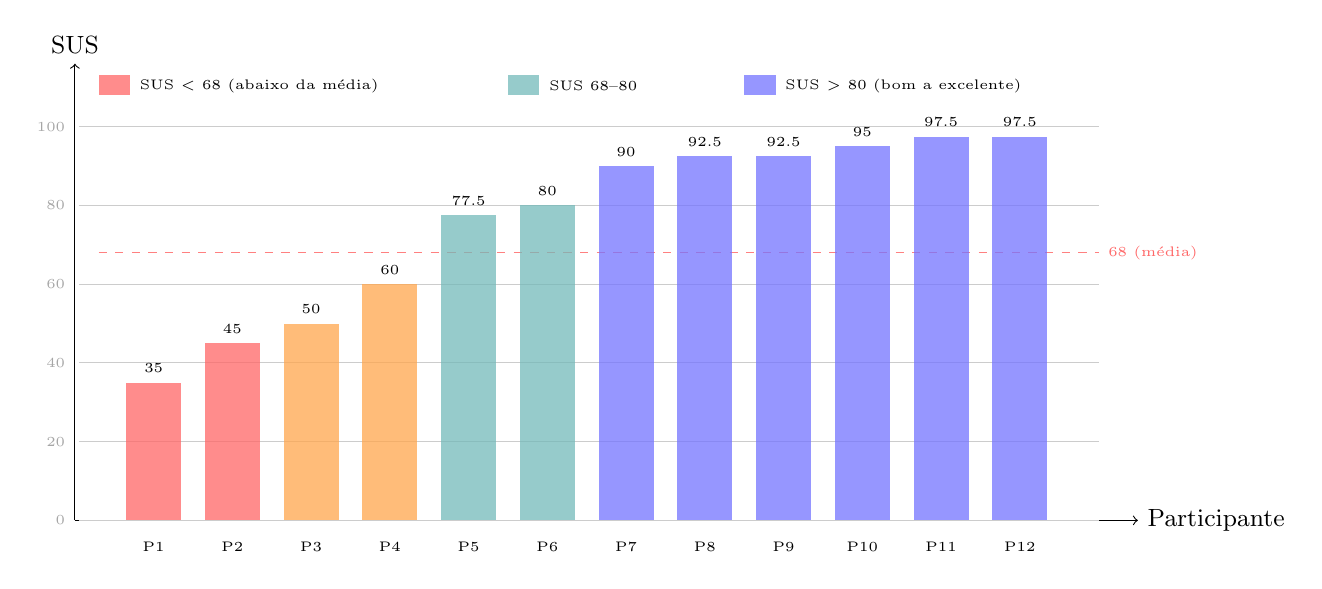
\begin{tikzpicture}[scale=1]
		\begin{scope}
			\draw[->] (0,0) -- (13.5,0) node[right, font=\small] {Participante};
			\draw[->] (0,0) -- (0,5.8)  node[above, font=\small] {SUS};

			\foreach \y/\label in {0/0, 1/20, 2/40, 3/60, 4/80, 5/100} {
				\draw[gray!40] (0.05,\y) -- (13,\y);
				\node[left, font=\tiny, gray!70] at (0,\y) {\label};
			}
			\draw[dashed, red!50, thin] (0.3,3.4) -- (13,3.4)
				node[right, font=\tiny, red!60] {68 (média)};

			\def\bw{0.7}
			\foreach \i/\sus/\col in {
				1/35/red!60,
				2/45/red!60,
				3/50/orange!70,
				4/60/orange!70,
				5/77.5/teal!55,
				6/80/teal!55,
				7/90/blue!55,
				8/92.5/blue!55,
				9/92.5/blue!55,
				10/95/blue!55,
				11/97.5/blue!55,
				12/97.5/blue!55
			} {
				\pgfmathsetmacro{\h}{\sus * 0.05}
				\fill[\col, opacity=0.75]
					(\i - \bw/2, 0) rectangle (\i + \bw/2, \h);
				\node[font=\tiny, above] at (\i, \h) {\sus};
			}
			\foreach \i in {1,...,12} {
				\node[font=\tiny, below] at (\i, -0.15) {P\i};
			}
			\fill[red!60, opacity=0.75]   (0.3, 5.4)  rectangle (0.7, 5.65);
			\node[right, font=\tiny] at (0.7, 5.52)  {SUS $<$ 68 (abaixo da média)};
			\fill[teal!55, opacity=0.75]  (5.5, 5.4)  rectangle (5.9, 5.65);
			\node[right, font=\tiny] at (5.9, 5.52)  {SUS 68--80};
			\fill[blue!55, opacity=0.75]  (8.5, 5.4)  rectangle (8.9, 5.65);
			\node[right, font=\tiny] at (8.9, 5.52)  {SUS $>$ 80 (bom a excelente)};
		\end{scope}
	\end{tikzpicture}
	\caption[Distribuição das pontuações SUS por participante (valores exatos do CSV)]{Pontuações SUS individuais dos 12 participantes, calculadas a partir das respostas brutas do CSV e ordenadas de forma crescente. Os valores são exatos (e.g., 77,5; 92,5; 97,5) sem arredondamento. A linha a tracejado assinala o limiar histórico de 68 pontos.}
	\label{fig:sus-distribuicao}
\end{figure}

A análise por questão SUS (Tabela~\ref{tab:sus-por-questao}) mostra que a plataforma é percepcionada como \textbf{fácil de usar} (Q3: 4,25) e \textbf{confiante de operar} (Q9: 4,25), com funções \textbf{bem integradas} (Q5: 4,00). Os itens mais penalizadores são a \textbf{intenção de uso frequente} (Q1: 3,67) e a \textbf{velocidade de aprendizagem} (Q7: 3,67) --- a barreira de entrada é baixa, mas o incentivo de regresso não é suficientemente robusto.

\begin{table}[htbp]
	\centering
	\small
	\begin{tabular}{c p{6.5cm} c r}
		\toprule
		\textbf{Q\#} & \textbf{Formulação (resumida)} & \textbf{Pol.} & \textbf{Média} \\
		\midrule
		Q1  & Usaria frequentemente                 & $+$ & 3,67 \\
		Q2  & Desnecessariamente complexo            & $-$ & 2,17 \\
		Q3  & Fácil de usar                         & $+$ & \textbf{4,25} \\
		Q4  & Precisaria de suporte técnico         & $-$ & \textbf{1,75} \\
		Q5  & Funções bem integradas                & $+$ & 4,00 \\
		Q6  & Demasiada inconsistência              & $-$ & \textbf{1,67} \\
		Q7  & A maioria aprenderia rapidamente      & $+$ & 3,67 \\
		Q8  & Pesado de usar                        & $-$ & \textbf{1,83} \\
		Q9  & Confiante a usar                      & $+$ & \textbf{4,25} \\
		Q10 & Precisou aprender muito antes         & $-$ & 2,00 \\
		\bottomrule
	\end{tabular}
	\caption[Médias por questão da SUS calculadas a partir dos dados brutos do CSV ($n=12$)]{Médias por questão da \emph{System Usability Scale} calculadas a partir das respostas brutas do CSV. Pol.~= polaridade da questão. Em negrito os itens mais salientes positiva e negativamente. $n=12$.}
	\label{tab:sus-por-questao}
\end{table}

A clivagem bimodal não corresponde à afiliação institucional: P05 (Alumni ISEL, SUS~35) e P09 (Estudante ISEL, SUS~60) ficaram no Grupo~B, enquanto vários utilizadores externos obtiveram SUS acima de 90 (Grupo~A). O agrupamento é comportamental:

\begin{itemize}
	\item \textbf{Grupo~A} ($n=8$, SUS médio 89,4): adoptaram a plataforma com entusiasmo; completaram 1 a 3 tópicos; mantiveram \emph{streaks} de 5 a 13 dias; sentiram o ciclo de erro como oportunidade de aprendizagem. Os 12 percursos adaptativos de P2 mostram que errar com frequência, mas persistir, é o perfil típico deste grupo.
	\item \textbf{Grupo~B} ($n=4$, SUS médio 47,5): a plataforma digital constitui, em si mesma, uma barreira --- \emph{``Because it's so confusing, it ends up not being so helpful, what would make people lose interest in this app and also patience''} (P04). Não concluíram nenhum tópico; \emph{streaks} de 1 a 3 dias. O problema não é o conteúdo, é o meio: a aprendizagem autónoma por aplicação web pressupõe um grau mínimo de familiaridade digital que este grupo ainda não possui.
\end{itemize}

\begin{table}[htbp]
	\centering
	\small
	\begin{tabular}{p{4cm} p{4cm} p{4cm}}
		\toprule
		\textbf{Dimensão} & \textbf{Grupo A} (\emph{n}~=~8) & \textbf{Grupo B} (\emph{n}~=~4) \\
		\midrule
		SUS médio           & 89,4 (Bom/Excelente)       & 47,5 (Mau) \\
		Amplitude SUS       & 77,5~--~97,5               & 35~--~60 \\
		Afiliação           & Misto (Ext.~+~ISEL)        & Misto (Ext.~+~ISEL) \\
		Tópicos concluídos  & 1~--~3 por utilizador      & 0 \\
		\emph{Streak} máx.  & 5~--~13 dias               & 1~--~3 dias \\
		Reação ao ciclo IA  & ``Fascinante e útil''      & Fluxo não percebido \\
		Envolvimento real   & Alto e sustentado          & Abandonado cedo \\
		\bottomrule
	\end{tabular}
	\caption[Comparação dos dois grupos de utilizadores identificados]{Síntese dos dois grupos de utilizadores, identificados pelo desempenho SUS e pelos dados comportamentais da BD. O agrupamento é comportamental, não por papel/afiliação.}
	\label{tab:dois-grupos}
\end{table}

O feedback qualitativo revelou três temas recorrentes: (1)~\textbf{ciclo de feedback por IA} como melhor funcionalidade, mencionado espontaneamente por 7 dos 11 respondentes à questão aberta (\emph{``The fact that when we get an answer wrong, artificial intelligence tries to help us understand why we got it wrong''} --- P02; \emph{``AI adaptability to your answers''} --- P12); (2)~\textbf{funcionalidades sociais e comunitárias} --- comparação de progressos com amigos, ``rivalidade positiva'' (P01, P09, P11), directamente alinhado com a dimensão de \emph{relação} da Teoria da Autodeterminação~\cite{deci1985intrinsic}; (3)~\textbf{consistência da interface} --- títulos mistos PT/EN, ausência de explicação quando a questão muda após um erro, e respostas da IA longas para ecrã de telemóvel.

% ─────────────────────────────────────────────────────────────────────────────
\subsection{O ciclo adaptativo em ação: um exemplo real}
\label{sec:dois-grupos}\label{ssec:dois-grupos}\label{ssec:exemplo-conversa}
% ─────────────────────────────────────────────────────────────────────────────

A sessão de explicação mais extensa registada na BD (8 trocas, \texttt{RESOLVED}, $\approx$3 minutos) ilustra o princípio de \emph{step-level feedback}~\cite{vanlehn2011relative}. O conteúdo e o diálogo apresentados abaixo estão em inglês porque essa é a língua de trabalho da plataforma --- uma escolha deliberada dado o público internacional do projecto no âmbito da aliança U!REKA~\citep{ureka2026alliance} --- apesar de o presente relatório ser redigido em português. O utilizador realizava \emph{Sustainable Cities \& Civic Engagement} e a submissão tinha sido classificada pelo sistema como \texttt{READING\_ERROR}.

\medskip
\noindent\textbf{A tarefa original:}
\begin{quote}
\small\itshape
\emph{``A digital device is a tool that uses electronic signals to process, store, or send information. Examples include phones, computers, and tablets. --- Which of the following is NOT a digital device? A) A calculator that adds numbers. B) A microwave that shows time. C) A toaster that pops up bread. D) A smartphone that plays music.''}
\end{quote}

\smallskip
\noindent\textbf{Diálogo de explicação:}

\begin{sloppypar}
\begin{description}
	\item[\small USER] \small \emph{``Why is my answer wrong?''}
	\item[\small AI]   \small \emph{``Could you share the exact sentence or paragraph you wrote? That way I can see exactly where the misunderstanding is and help fix it.''}
	\item[\small USER] \small \emph{``A smartphone that plays music is a digital device''}
	\item[\small AI]   \small \emph{``Ah, I see the confusion! A smartphone playing music is indeed a digital device, but the question is about digital public services \textnormal{[...]}. Think of it this way: your smartphone is just the tool --- digital public services are the services that run on those tools to make cities greener. Does that help clarify the difference?''}
	\item[\small USER] \small \emph{[partilha o enunciado completo e indica que C é a resposta correta]}
	\item[\small AI]   \small \emph{``Ah, now I see the mix-up! The clue is in the definition: a digital device has to process, store, or send information. A toaster just heats bread --- it doesn't do any of those things, so it's not digital. But a smartphone plays music by processing data, so it is digital. Does that make sense now?''}
	\item[\small USER] \small \emph{``Yes, then why is C right and not D?''}
	\item[\small AI]   \small \emph{``A toaster pops up bread because a timer inside it has counted down; that timer is a tiny computer storing and counting `ticks,' so it does process and store information. A smartphone playing music is also digital, but the question lets only one answer be chosen, and the hint wants the simplest device that still fits the definition.''}
\end{description}
\end{sloppypar}

\medskip
A IA não deu a resposta de imediato: solicitou que o utilizador explicitasse a sua dúvida, escalou a explicação quando a confusão persistiu, e a última troca mostra que o utilizador chegou a um nível de compreensão suficiente para formular a dúvida correta --- já não estava perdido, estava a refinar. Toda a sessão decorreu em \textbf{menos de 3 minutos}.

Este exemplo ilustra também, de forma concreta, a limitação do \texttt{ErrorPatternClassifier} discutida na Secção~\ref{ssec:padroes-erro}: a heurística posicional classificou esta submissão como \texttt{READING\_ERROR}, mas o diálogo revela uma confusão conceptual genuína sobre o que qualifica um dispositivo como ``digital'' (o critério de processar/armazenar/transmitir informação, não a familiaridade do objecto do dia-a-dia) --- mais próxima, em substância, de um \texttt{WRONG\_CONCEPT}. O caso confirma que a heurística estrutural nem sempre corresponde à natureza real do erro cometido.

% ─────────────────────────────────────────────────────────────────────────────
\subsection{Limitações}
\label{ssec:discussao-f2}
% ─────────────────────────────────────────────────────────────────────────────

Esta avaliação tem limitações que devem ser explicitamente reconhecidas:

\begin{itemize}
	\item \textbf{Dimensão da amostra} ($n=12$): insuficiente para conclusões estatisticamente robustas; os resultados devem ser lidos como indicadores preliminares.
	\item \textbf{Amostragem por conveniência}: pode sobre-representar utilizadores com familiaridade digital, ampliando o Grupo~A e subestimando o Grupo~B.
	\item \textbf{Dados comportamentais do último ciclo}: o \emph{snapshot} da BD cobre o período após o último \emph{reset} de desenvolvimento, não a totalidade histórica do projeto; sem grupo de controlo, não é possível atribuir causalmente os resultados à plataforma.
	\item \textbf{Ausência de validação pedagógica}: nenhum tópico foi revisto por especialistas em educação cívica; a qualidade factual do conteúdo gerado pelo LLM depende da qualidade dos \emph{prompts} e do modelo, e não foi avaliada de forma independente.
	\item \textbf{Validade do classificador de padrões de erro não estabelecida}: o \texttt{ErrorPatternClassifier} usa uma heurística puramente posicional para distinguir \texttt{READING\_ERROR} de \texttt{WRONG\_CONCEPT} (Secção~\ref{ssec:padroes-erro}), sem validação contra um \emph{ground truth} humano; o exemplo da Secção~\ref{ssec:exemplo-conversa} mostra um caso em que a classificação automática não correspondeu à natureza real do erro.
	\item \textbf{Correspondência entre amostras}: a análise cruzada entre pontuação SUS e comportamento na BD (Secção~\ref{ssec:sus}) assume que a identificação do utilizador no momento de resposta ao questionário foi feita de forma fiável; um pequeno desvio nessa associação não foi independentemente re-verificado para este relatório.
\end{itemize}

Apesar destas limitações, a triangulação entre questionário e dados comportamentais --- sustentada pela integridade do sistema demonstrada em §\ref{sec:integridade-geracao} --- permitiu uma leitura mais completa do que cada fonte isolada: os dados de utilização confirmam hipóteses levantadas pelo questionário, e as respostas qualitativas explicam padrões visíveis nos dados de comportamento.
